\newcommand{\seccion}{SECUNDARIA INCORPORADA A LA SEG }
\newcommand{\descripcion}{Examen Parcial, Segundo Bimestre}
\newcommand{\grado}{Primero de secundaria}
\newcommand{\ciclo}{Ciclo escolar: 2015--2016}
\newcommand{\papel}{legalpaper} %letter, legalpaper ...
\newcommand{\fecha}{24 de noviembre de 2015}
% \author{Ing. Arturo Canedo \\ M. en C. Reinaldo Zapata}
\author{M. en C. Reinaldo Zapata}

\documentclass[11pt]{article}
\usepackage[\papel]{geometry}

\title{\flushleft \seccion \\ \descripcion \\  \grado \\ \ciclo}

\newcommand\BackgroundLogo{
\put(162,365){
\parbox[b][\paperheight]{\paperwidth}{%
\vfill
\centering
\includegraphics[width=5cm,height=2.5cm,keepaspectratio]{/Users/reinaldo/Documents/clases/jassa/logo}%
\vfill
}}}



% \title{\seccion \\ \descripcion \\  \grado \\ \ciclo}

% \newcommand\BackgroundLogo{
% \put(162,435){
% \parbox[b][\paperheight]{\paperwidth}{%
% \vfill
% \centering
% \includegraphics[width=5cm,height=2.5cm,keepaspectratio]{/Users/reinaldo/Documents/clases/jassa/logo}%
% \vfill
% }}}

\hyphenation{con-ti-nua-ción}

\usepackage{enumitem}
\usepackage[T1]{fontenc} %fuentes
\usepackage{lmodern} %fuente mejorada
\usepackage[spanish]{babel}
\decimalpoint
\usepackage{fullpage}
\usepackage{multicol}
\usepackage{graphicx}
\usepackage{eso-pic}
\usepackage{multirow}
\usepackage{subfigure}
\usepackage{tikz}


%Modificación del formato de las ecuaciones y el numerado de las mismas
\usepackage[leqno,fleqn]{amsmath}
\makeatletter
  \def\tagform@#1{\maketag@@@{#1\@@italiccorr}}
\makeatother
\renewcommand{\theequation}{\fbox{\textbf{\arabic{equation}}}}


\begin{document}
\AddToShipoutPicture*{\BackgroundLogo}
\ClearShipoutPicture
\date{\fecha}
\maketitle
% \thispagestyle{empty}


Nombre del alumno:\,\line(1,0){244}\,.\hspace*{.2cm} \hfill Aciertos:\,\line(1,0){35}\,. \\

\indent Primero de secundaria, grupo:\,\line(1,0){35}\,. No. de lista:\,\line(1,0){35}\,. \hfill 40 \quad \ 

\vspace{5mm}

El prop\'osito de todo examen es poner a prueba los conocimientos de cada alumno
para calificar as\'i su desempe\~no y aprendizaje. Contesta correctamente, en
cada secci\'on, tantos reactivos como te sea posible. Todas y cada una de las
operaciones deber\'as escribirlas en esta hoja donde se imprimi\'o el examen y
los resultados finales deber\'an estar escritos con tinta.

\section{Geometr\'ia}

Calcula el \'area del tri\'angulo si se tiene que la longitud de su base es
$b=5$\,cm y la de su altura es $h=4.8$\,cm. (valor: 4 aciertos.)

\begin{figure}[h!]
        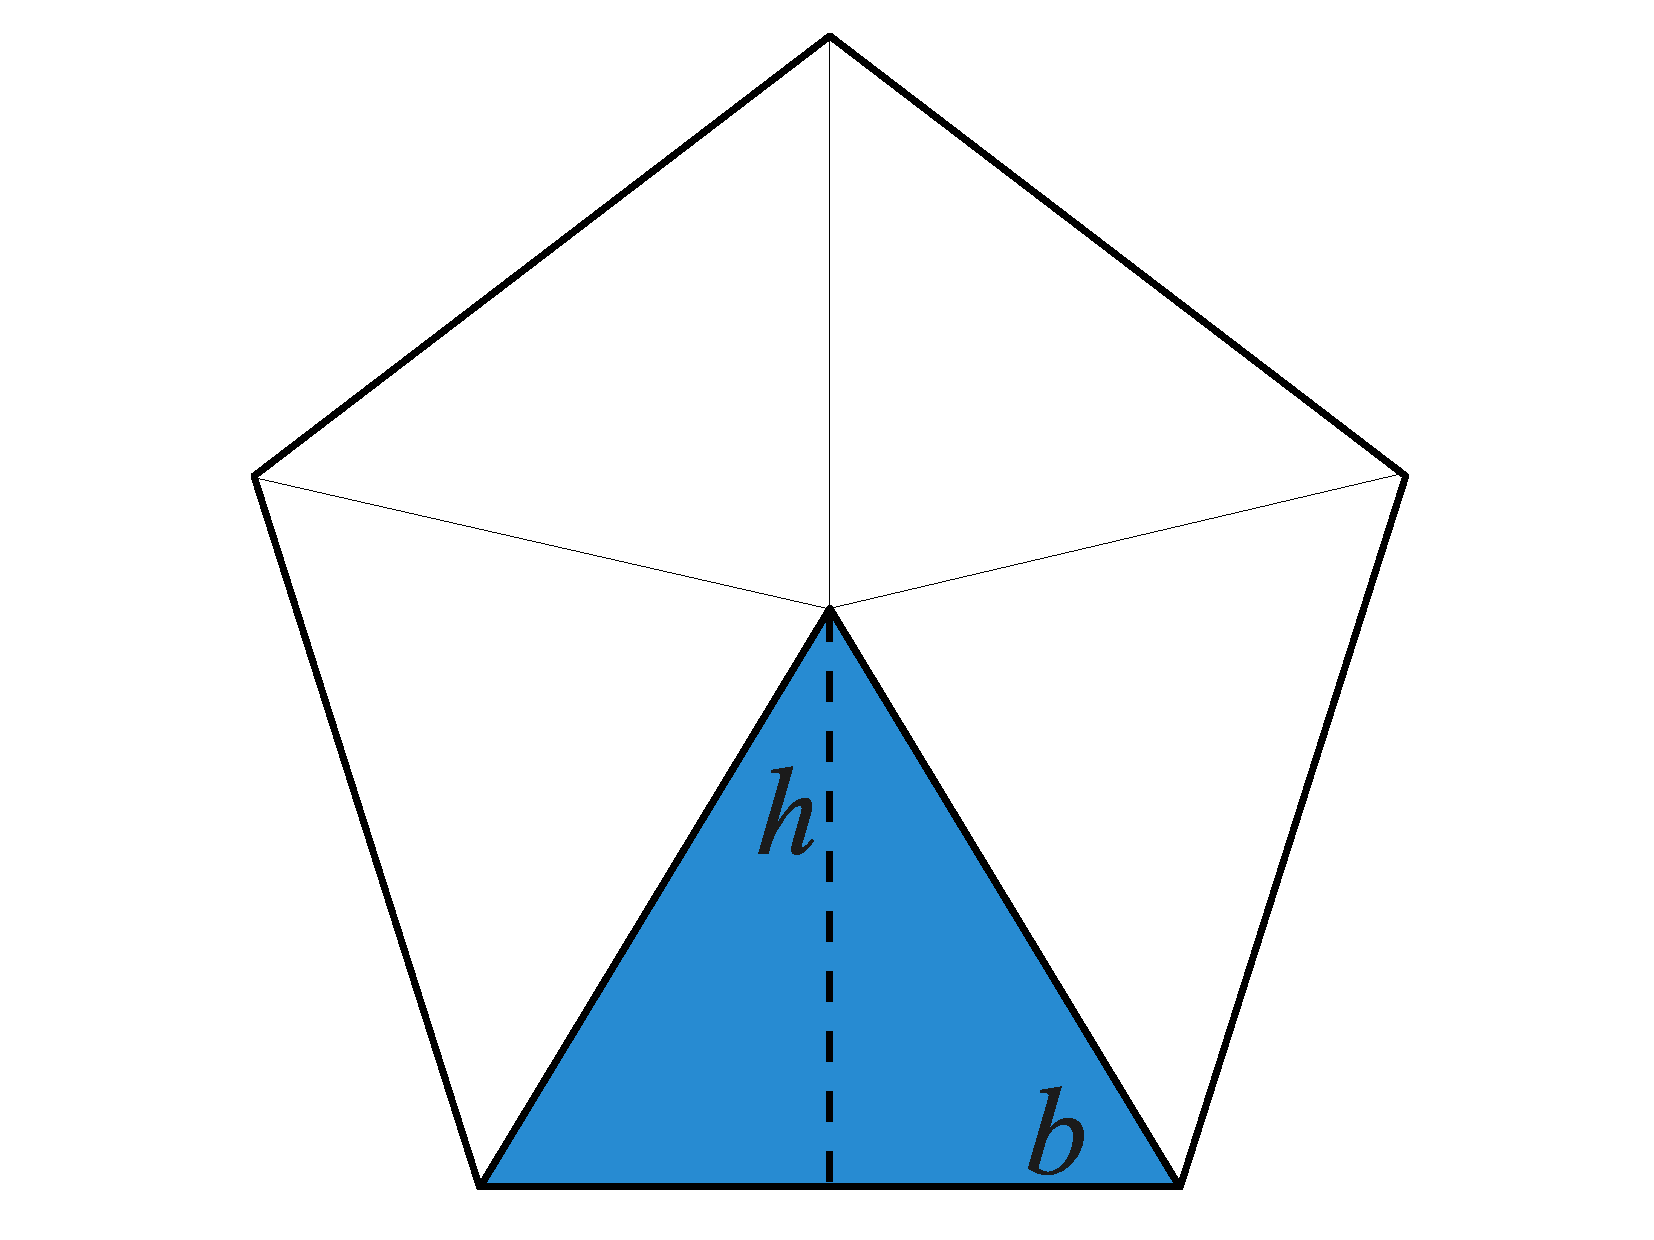
\includegraphics[width=0.32\textwidth]{./pentagono}
    \label{fig:granja}
\end{figure}


Observando la figura previa date cuenta cuantos tri\'angulos al sombreado
conforman al pent\'agono. Bas\'andote en ello y en tu resultado anterior calcula
su \'area. (valor: 4 aciertos.)

\vspace{3cm}

En la siguiente figura se muestra un rect\'angulo. Se tiene que la longitud de
su base es $b=\frac{11}{4}$\,km y su altura es $h=\frac{6}{5}$\,km. Usando
fracciones calcula su per\'imetro. (valor: 4 aciertos.)

\begin{figure}[h!]
        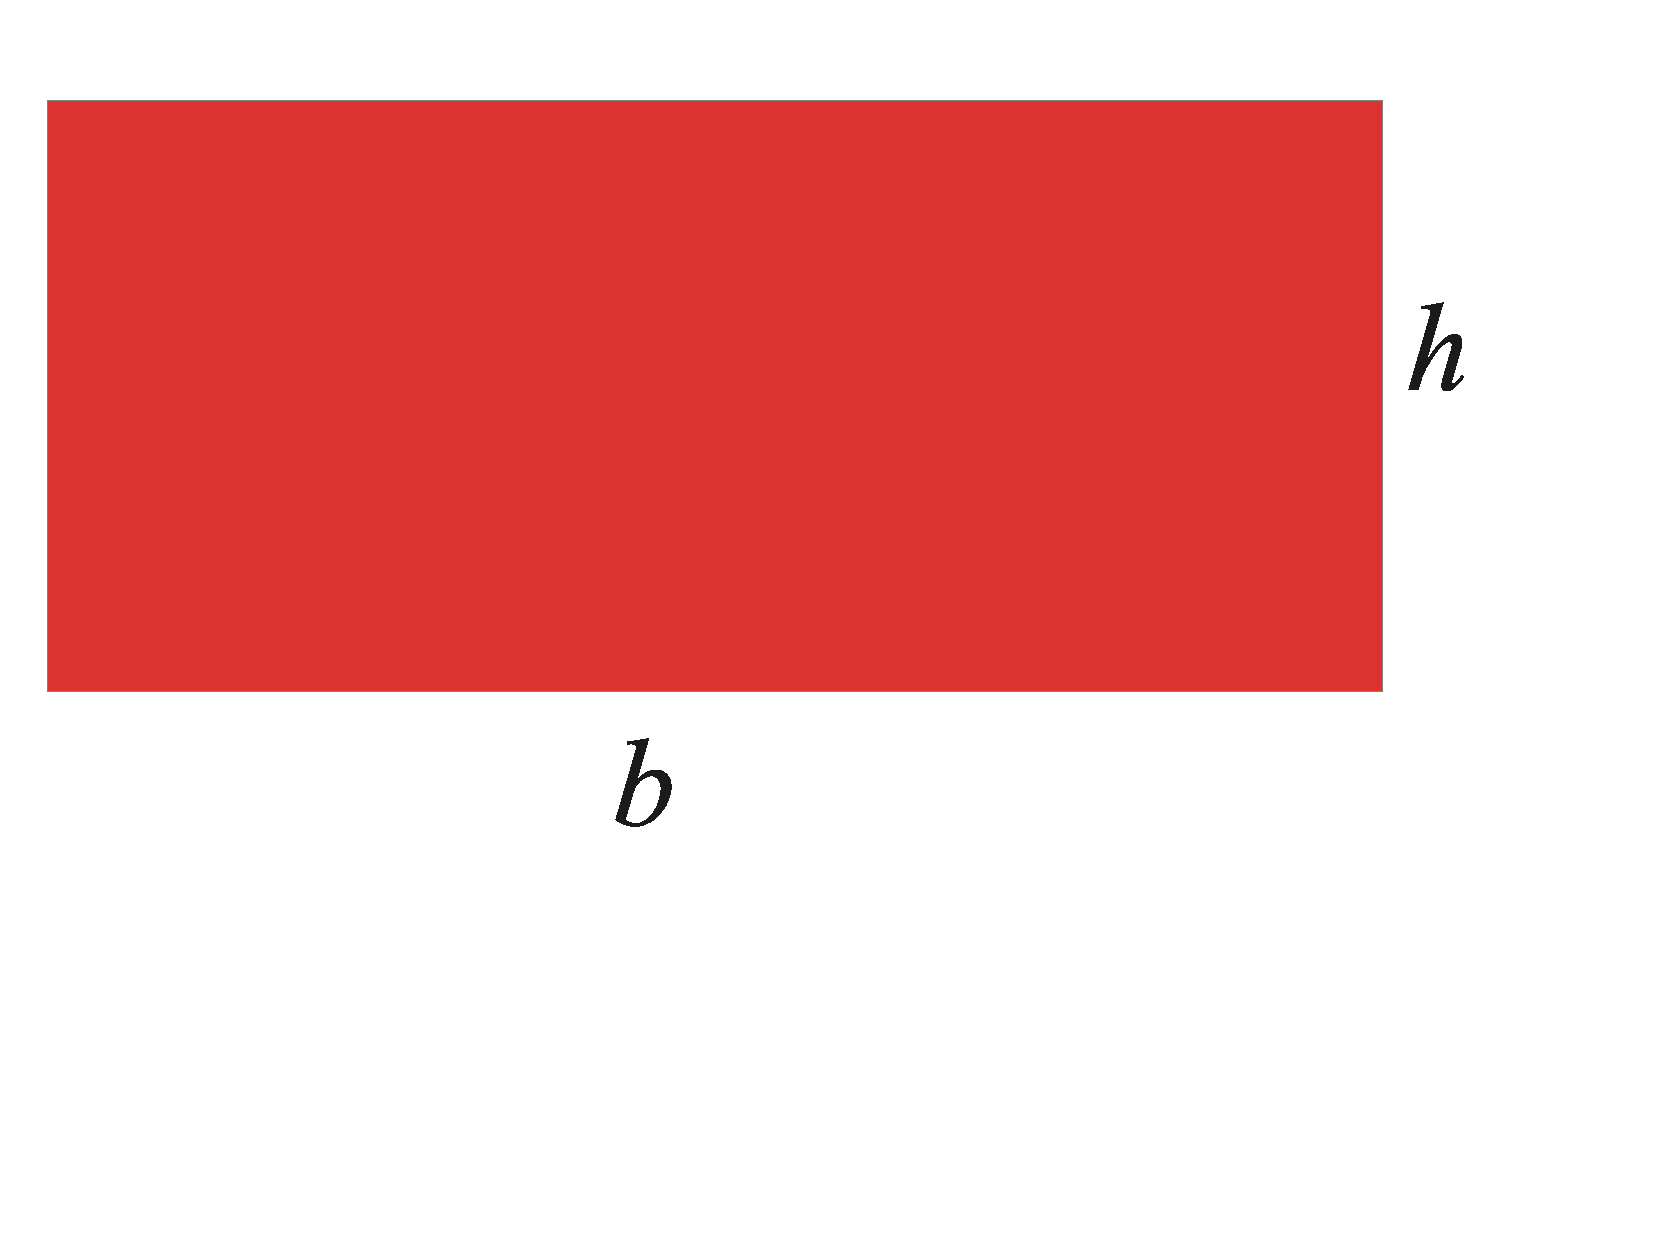
\includegraphics[width=0.32\textwidth]{./rectangulo}
    \label{fig:rectangulo}
\end{figure}

\newpage

Partiendo de los datos de la figura anterior convierte los valores de la base y
la altura a decimales. Usando estos nuevos datos calcula su \'area. (valor: 4
aciertos.)

\vspace{5cm}

\section{Proporcionalidad y regla de tres}

Resuelve los problemas que se plantean a continuaci\'on.

\vspace{0.5cm}

Como promoci\'on en un supermercado se tiene que el costo de medio kilogramo de
manzana es \$9.50. ?`Cu\'anto se deber\'a pagar por cuatro kilogramos de
manzana? (valor: 2 aciertos)

\vspace{5cm}

Dise\~nado para alcanzar una gran velocidad,  el auto deportivo
\textit{Lamborghini Veneno} alcanza una velocidad m\'axima de 221 millas por
hora. Sabiendo que una milla equivale a 1.609 kil\'ometros, determina dicha
velocida en kil\'ometros por hora. (valor: 3 aciertos)

\vspace{5cm}

Para cierta venta especial en una tienda departamental se tienen descuentos del
50\% + 10\%. Aprovechando esa oportunidad el profesor de matem\'aticas decide
comprar una playera tipo polo. Si el precio original de la playera era de
\$899.00,  determina el costo final que el profesor pagar\'a por dicho
art\'iculo. (valor: 5 aciertos)

\newpage

\section{Introducci\'on al \'algebra}


Completa la tabla que se muestra a continuaci\'on separando las expresiones
algebraicas en sus respectivos componentes. (valor: 4 aciertos.)

\begin{center}
{\large
\begin{tabular}{|c|c|c|c|}
\hline
Expresi\'on & Coeficiente & Literal(es) & Exponente(s)  \\ \hline 
\Large $3x^2$ &&&\\ \hline
\Large $b^2c^4x^6$ &&&\\ \hline
\Large $17ax^2y^3$ &&&\\ \hline
\Large $d^2we^3x$ &&&\\ \hline
\end{tabular}
}
\end{center}

Haz la reducci\'on de los t\'erminos semejante de la forma como se trabaj\'o en
clase. (valor: 10 aciertos.)

\begin{equation*}
3m + 20p + 5m - 6p = 
\end{equation*}
\begin{equation*}
5p + m -p +2m + 6p =
\end{equation*}
\begin{equation*}
8p + m -5p + 12m + 2p + 2m =
\end{equation*}
\begin{equation*}
3x + 4y - x = 
\end{equation*}
\begin{equation*}
20x + 17y - 8x - y -3x =
\end{equation*}

\end{document}






